\section{Ejercicio 9}
En esta parte del trabajo se nos pidi\'o el an\'alisis de concepto de \textit{fairness} del algoritmo de scheduling \texttt{SchedLottery}. Tomamos como definici�n de \textit{fairness}, al hecho de que cada
proceso reciba igual cantidad de tiempo de CPU, o m�s precisamente, un tiempo apropiado para
cada proceso de acuerdo a su prioridad y carga de trabajo.

\vspace{2mm}

La medici\'on de \textit{fairness} se basa en el concepto de promedio de tickets. De un lote de tareas id\'enticas, realizamos $n$ simulaciones, de las cuales analizamos los primeros $k$ ticks. Durante estos $k$ ticks, medimos la cantidad de ticks que fue asignada cada tarea. 

\vspace{2mm}

Consideramos que un scheduler es justo, si durante esos $k$ ticks analizados, si cada tarea tiene un n\'umero asignado de ticks similar. Lo considerari\'iamos completamente justo si, habiendo $i$ tareas, cada tarea reciba $k/i$ de ticks. Nos bastar\'a ver que se acerce a ese n\'umero para considerarlo justo. Notar que, $k$ debe ser menor a la duraci\'on de las tareas, ya que de otra forma, si las tareas finalizan en menos de $k$ ticks, cada tarea recibi\'o todos los ticks que necesitaba y no puede analizarse nada relevante.

\vspace{2mm}

Dada la naturaleza pseudoaleatoria del \texttt{SchedLottery}, no basta una sola simulaci\'on, ya que puede ser arbitrariamente injusta. Nuestra forma de ver que la cantidad de ticks asignados a cada tarea en el per\'iodo de $k$ ticks, es hacer sucesivas simulaciones, y tomar el promedio de ticks asignados a cada tarea. Luego de un n\'umero de $n$ simulaciones, esperamos ver que el promedio de estos ticks asignados a cada tarea se acerque a $k/i$.

\vspace{2mm}

\subsection{Par\'ametros de experimento}

\vspace{2mm}

El lote a analizar es el siguiente:

\begin{lstlisting}[numbers=none]
@0:
*5 TaskCPU 100
\end{lstlisting}

\vspace{2mm}

La cantidad de tareas a analizar van a ser 5, de forma de tener suficientes para comparar, pero que no resulte tan complejo el an\'alisis. La cantidad de ticks a analizar $k$ es 250, para realizar de forma m\'as sencilla el c\'alculo $k/i$, esperaremos que cada tarea reciba aproximadamente 50 ticks.

\vspace{2mm}

La elecci\'on de 5 tareas de CPU se basa en la simplicidad de la medici\'on de la asignaci\'on justa, ya que no hay que considerar casos de bloqueos ni de tickets compensatorios que hagan m\'as complejo el an\'alisis de la asignaci\'on. Cada tarea dura 100 ticks, de forma de asegurarnos que no terminen antes de los $k$ ticks.

\vspace{2mm}

Por \'ultimo, luego de realizar varias series de simulaciones, notamos que con la cantidad de experimentos $n=1000$ puede verse claramente la tendencia del promedio de los ticks.

\vspace{2mm}

\subsection{Gr\'afico de resultados del experimento}

\begin{center}
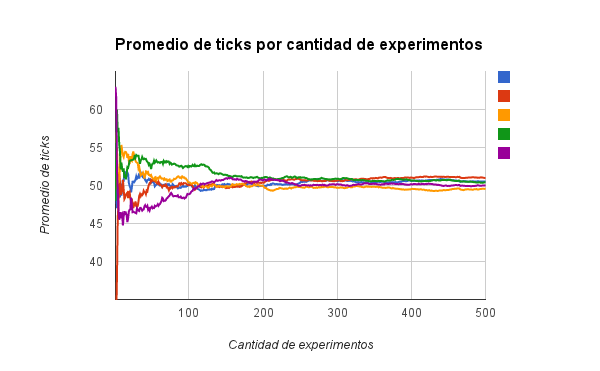
\includegraphics[scale=0.8]{./Graficos/ej10.png}
\end{center}

Siendo $k/i=50$, puede notarase claramente que luego de sucecivas simulaciones, el promedio de ticks se acerca efectivamente al n\'umero esperado.

\vspace{2mm}

\textbf{Nota:} los detalles de la simulaci\'on pueden verse en el script de bash $run_experiments9.sh$.